%----------------------------------------------------------------------------
\chapter{The paper, chapter by chapter}\label{app:chapters}
%----------------------------------------------------------------------------
Your chapter files start nearly empty: the headings of the paper, an orange note under each that links here, the running-example boxes, one item of each tagged list, and stubs of the figures and tables the lint looks for. This chapter holds the rest. It follows the files' headings one by one, and for each it gives what the reviewer scores there, the beat of its paragraph (\cref{app:writing:spine}), and the items in action, written for the guide's own running example, \exname. Read a section before you write the matching part of your paper. Copy what you need from the source, \texttt{guide/chapter-by-chapter.tex}, and drop the \texttt{guide:} part of every label you copy, so that \texttt{req:guide:offline} becomes \texttt{req:offline}.

The paper sketched here is made up, and it is the same paper as the mind map of \cref{fig:mindmap}. Its approaches A to D, its numbers and its results show what each item looks like when it is finished; none of them describes a real system.

\paragraph{What the reviewer scores.} The review sheet (\cref{app:tdk:sheet}) gives 35 points: A form and style 0--5 (30--35 pages; about 1 point off per 3 pages outside that range), B figures and literature 0--4, C topic 0--8, D originality and soundness 0--10, E introduction and evaluation 0--8. Argue four things throughout the paper; each section below says which of them its chapter carries, and quotes the criterion in the sheet's words.
\begin{description}[noitemsep]
  \item[Relevance (C)] The topic matters now.
  \item[Non-triviality (C and D/1)] Solving it takes deep or scientific knowledge, not a textbook recipe or a copy of known solutions.
  \item[Novelty (D/1)] Full marks for a solution that is new at least in Hungary or does not exist yet; an incremental improvement earns 3--4 of 5.
  \item[Correctness (D/2)] Every result is backed and checkable.
\end{description}
Criterion A is scored on the whole paper: \enquote{4--5: kiváló (ha a dolgozat közel hibamentes, jól tagolt, követhető, gördülékeny stílusú)}, and \enquote{Terjedelmi korlát 30--35 oldal. Ettől eltérés esetén 3 oldalanként 1 pont levonás javasolt.}

\paragraph{What a skimming reviewer reads.} A reviewer with a stack of papers reads the headings, the abstract, the tagged items (C1, REQ1, AS1, SG1, \dots), the theorems, the running-example boxes, and the figures and tables with their captions; a paragraph registers only as so many lines of text. A heading marked \skimmark{} below holds such an item. An unmarked one holds paragraphs only, so the claim it makes must also show in a marked item, in a caption, or in the heading itself.

%----------------------------------------------------------------------------
\section{Introduction}\label{app:chapters:intro}
%----------------------------------------------------------------------------
\textbf{Criteria C and E.} A reviewer who reads only the introduction and its leading figure should be able to say what you did and why it matters.
\textbf{Relevance:} open with why the problem matters now and to whom.
\textbf{Non-triviality:} show why the obvious solutions fail.
\textbf{Novelty:} state the contributions as checkable claims.

\textbf{In the sheet's words.} The top of C: \enquote{7--8: tudományos vizsgálat szükséges (ha a dolgozat témája korszerű, nem lezárt, vizsgálata magas szintű, tudományos, elmélyült tudást igényel)}. The bottom of E names what this chapter must contain: \enquote{0: teljesen hiányzik -- ha a dolgozat bevezetése hiányos (tématerület áttekintése, problémafelvetés, fő kontribúció kimondása)}.

\subsection{Context}\label{app:chapters:context}
\guidebeat{why the field matters now}{a trend, a regulation or an incident, cited}{not yet introduced}{the problem}
Every abbreviation goes through \texttt{\textbackslash gls}, as in \gls{vc}, which spells it out on first use; declare it in \texttt{content/glossary.tex}, together with the paper's notation and terms.

\subsection[Problem]{Problem\skimmark}\label{app:chapters:problem}
\guidebeat{the concrete problem, ending in a one-sentence problem statement}{the running example}{introduced here: who the actors are, what they want to do, and what goes wrong}{the requirements}
The box introduces the running example in two or three sentences: the actors, what they want to do, and what goes wrong today. Every chapter returns to it, so choose a scenario small enough to follow and rich enough to show every requirement.
\begin{runningexample}
A university issues a diploma to a graduate as a verifiable credential, and later revokes it because the degree was withdrawn. An employer checks the diploma during hiring and accepts it: its copy of the revocation status is a day old.
\end{runningexample}

\subsection[Requirements]{Requirements\skimmark}\label{app:chapters:requirements}
\guidebeat{what a solution must do}{one requirement per failure of the example; they are the rows of the gap matrix and the yardstick of the evaluation}{the part of the scenario each requirement comes from}{the gap}
Each requirement is a property the running example needs, stated so it can be checked. Usually one of them is what existing approaches trade off against the others.
\begin{requirements}
  \item\label{req:guide:timely} \textbf{Timely revocation.} Every verifier sees a revocation within $\delta$ of its submission.
  \item\label{req:guide:offline} \textbf{Offline checks.} A verifier checks a credential without contacting its issuer.
  \item\label{req:guide:private} \textbf{Holder privacy.} A check tells nobody, the issuer included, which credential was checked.
\end{requirements}

\subsection{Gap, in brief}\label{app:chapters:introgap}
\guidebeat{that no existing approach meets the requirements together; the full comparison comes after the evaluation (\cref{ch:related}), so this paragraph carries the novelty claim on its own}{the closest approaches, cited}{what the closest approach does with the example, and where it fails}{the contributions}
Name the closest approaches and say which requirement each gives up. Here: asking the issuer at every check is timely but neither offline nor private, and offline lists are private but a day stale.

\subsection[Leading figure]{Leading figure\skimmark}\label{app:chapters:leading-figure}
\textbf{Criterion B/1} is scored on figures like this one. Well thought out means: the reader takes away one thing, the caption explains it (\cref{app:writing:captions}), and it is vector (\cref{app:writing:figures}). It should be understandable without the text, and what is yours must be visible at a glance (\cref{app:writing:figure}).

\textbf{In the sheet's words.} \enquote{4: kiváló (a dolgozat megfelelő számú és jól átgondolt ábrát, táblázatot tartalmaz, és a szakirodalmi hivatkozások pontosak)}; the step below is \enquote{2: átlagos (a dolgozat megfelelő számú ábrát és táblázatot tartalmaz, ám azok több esetben nem jól átgondoltak vagy rossz minőségűek)}.

\begin{figure}[!ht]
  \centering
  \begin{tikzpicture}[
      node distance=6mm and 10mm,
      col/.style={draw, rounded corners, minimum width=38mm, minimum height=26mm, align=center, font=\small},
      part/.style={ours, rounded corners=1pt, minimum width=34mm, minimum height=7mm, align=center, font=\footnotesize},
      lbl/.style={font=\small\bfseries, above=1mm}]
    \node[col, problem]   (problem) {A revoked diploma\\[1mm]\footnotesize is accepted, because\\\footnotesize the status is a day old};
    \node[part, right=12mm of problem, yshift=9mm] (c1) {C1: Registry model};
    \node[part, below=1.5mm of c1] (c2) {C2: Ledger registry};
    \node[part, below=1.5mm of c2] (c3) {C3: Evaluation};
    \node[draw=none, fit=(c1)(c3), inner sep=2mm] (approach) {};
    \node[col, result, right=of approach] (result) {Rejected within $\delta$\\[1mm]\footnotesize offline, and the issuer\\\footnotesize never learns who asked};
    \node[lbl] at (problem.north)  {Problem};
    \node[lbl] at (approach.north) {This work};
    \node[lbl] at (result.north)   {Evaluation};
    \draw[-Stealth, thick] (problem) -- (approach);
    \draw[-Stealth, thick] (approach) -- (result);
  \end{tikzpicture}
  \caption{Leading figure: the problem, the contributions, and the headline result in one picture. Blue is this work, every component of it in the same blue; the problem is red, the result green.}
  \label{fig:guide:overview}
\end{figure}

\subsection[Contributions]{Contributions\skimmark}\label{app:chapters:contributions}
\guidebeat{what this work claims, as checkable items with pointers to their support}{the chapters behind each contribution}{the leading figure shows the example solved}{the structure of the paper}
One item per contribution: a theoretical one (a model, formalisation, algorithm or protocol, with what it guarantees), a technical one (the tool, system or artifact that realises it), and the evaluation, each pointing to the chapter that delivers it.
\begin{contributions}
  \item\label{c:guide:model} \textbf{Registry model.} A formal model of revocation registries, and a proof that verifiers never accept a credential revoked more than $\delta$ ago (\cref{ch:approach}).
  \item\label{c:guide:registry} \textbf{Ledger registry.} A registry on a permissioned ledger where a check reads one accumulator witness, without asking the issuer, archived with its tests (\cref{ch:implementation}).
  \item\label{c:guide:eval} \textbf{Evaluation.} Correctness on the model and the scenario, scalability up to 10\,000 issuers, and robustness under node failures and load spikes (\cref{ch:evaluation}).
\end{contributions}

\subsection{Structure}\label{app:chapters:structure}
One sentence per chapter, in reading order. The paragraph in your introduction is already written; rename the chapters it lists when you rename them in the files.

%----------------------------------------------------------------------------
\section{Background}\label{app:chapters:background}
%----------------------------------------------------------------------------
\textbf{Criterion B/2.} Cite current research and industrial solutions, not only course material.
\textbf{Non-triviality:} introduce the concepts the hard part of \cref{ch:approach} relies on; textbook material gets a citation, not a re-derivation.
\textbf{Nothing of yours here.} This chapter is prior knowledge only, and every statement in it has a reference; the reader must be able to tell at the chapter boundary where the literature ends and your work begins.
\textbf{A companion paper.} When a TDK paper of the same year supplies what the approach builds on, the part this paper needs is restated here, condensed, and introduced as the companion paper's work without a citation (\cref{app:tdk:companion}). It is the one part of this chapter without a reference.

\textbf{In the sheet's words.} The scale for B/2 starts at \enquote{0: egyetemi tananyag (a dolgozat kizárólag egyetemi tankönyveket idéz kapcsolódó szakirodalomként)} and \enquote{1: ismert ipari gyakorlat (a dolgozat feldolgozta a weblapokról, technikai dokumentációkból közismert ipari megoldásokat)}; this chapter must already cite above that.

\subsection[First concept]{First concept\skimmark}\label{app:chapters:first-concept}
\guidebeat{the first concept the approach relies on; notation is defined once, here}{a definition and a citation}{the example expressed with this concept}{the second concept}
Name the section after the concept. The box restates the scenario of the introduction in this concept's vocabulary; the definition is precise enough for the later chapters to rely on.
\begin{runningexample}[in terms of verifiable credentials]
The diploma is a verifiable credential: the university is its \gls{issuer}, the graduate its \gls{holder}, and the employer a \gls{verifier}. The revocation is a second statement by the issuer, and the verifier must see it too.
\end{runningexample}
\begin{definition}[Verifiable credential]\label{def:guide:vc}
A \emph{verifiable credential} is a set of claims about a subject, signed by its issuer, that its holder can present to any verifier without the issuer taking part.
\end{definition}

\subsection{Second concept}\label{app:chapters:second-concept}
\guidebeat{the second concept}{a definition and a citation}{the example expressed with this concept}{the approach}
For the registry, the second concept would be the permissioned ledger the implementation stores revocations on: what it guarantees about history, and what it costs to append.

%----------------------------------------------------------------------------
\section{Approach}\label{app:chapters:approach}
%----------------------------------------------------------------------------
\textbf{Criteria D/1 and D/2 (0--10 together).} The core of the paper: your theoretical contributions, such as a model, formalisation, algorithm or protocol, and what it guarantees; \cref{ch:implementation} holds the technical ones. Rename the chapter after your method.
\textbf{Correctness:} every claim needs a proof, a mechanised proof, or a measurement; state assumptions explicitly.
\textbf{Novelty:} separate what is new from what you adopted from the literature.
\textbf{Non-triviality:} name the hard part and explain why the simple design does not work.
\textbf{Describe here, evaluate later.} This chapter states what the approach is and what it guarantees, objectively; how well it works is the evaluation's job, and praise here reads as a claim without evidence.

\textbf{In the sheet's words.} The top of D/1: \enquote{5: újszerű (legalább hazánkban újszerű, vagy eddig még nem létező megoldás)}; the top of D/2: \enquote{5: kiváló (kimagasló színvonalú kidolgozás, a közölt eredmények helyessége kétségkívül megalapozott)}.

\subsection[Overview]{Overview\skimmark}\label{app:chapters:overview}
\guidebeat{how the approach works end to end}{the architecture figure}{the example walked through the figure, component by component}{the model}
The box walks the scenario through the figure step by step: which component handles which part of it, and what each produces.
\begin{runningexample}[through the approach]
The university revokes the diploma at the registry service, which removes it from the accumulator and appends the new value, signed and timed, to the ledger. When the graduate presents the diploma with its witness, the employer's verifier library checks the witness against the newest signed value it holds, which must be younger than $\delta$. The revoked diploma's witness no longer verifies, and the diploma is rejected.
\end{runningexample}

\begin{figure}[!ht]
  \centering
  \begin{tikzpicture}[
      node distance=8mm and 14mm,
      comp/.style={draw, rounded corners, fill=blue!8, minimum width=28mm, minimum height=10mm, align=center, font=\small},
      ext/.style={comp, prior, dashed}]
    \node[ext]  (user) {Issuer};
    \node[comp, ours, right=of user] (core) {Registry service\\\footnotesize(contribution C2)};
    \node[comp, prior, right=of core] (store) {Permissioned ledger};
    \node[comp, ours, below=of core] (check) {Verifier library\\\footnotesize(contribution C2)};
    \draw[-Stealth] (user) -- node[above, font=\footnotesize]{revoke} (core);
    \draw[-Stealth] (core) -- node[above, font=\footnotesize]{append} (store);
    \draw[-Stealth] (core) -- node[right, font=\footnotesize]{signed value} (check);
    \begin{scope}[on background layer]
      \node[draw, dotted, inner sep=3mm, fit=(core)(store)(check), label={[font=\footnotesize]above right:System boundary}] {};
    \end{scope}
  \end{tikzpicture}
  \caption{Architecture of the registry. Blue components are this work, grey ones are reused or external: the issuer is outside the system, and the ledger is an existing product.}
  \label{fig:guide:architecture}
\end{figure}
In your paper, the stub in the approach chapter becomes this figure (\cref{fig:guide:architecture}): keep what is yours blue.

\subsection{Model or design}\label{app:chapters:model}
\guidebeat{the formal model or the design decisions}{each decision with the alternative rejected and why}{the example as an instance of the model}{the threat model}
Name the section after the model. For the registry: the revoked credentials as an accumulator, its values signed and timed on the ledger, a witness as the holder's proof that a credential is still in it, and the scenario's diploma as one element the revocation removes.

\subsection{Threat model and guarantees}\label{app:chapters:threat-model}
\guidebeat{who the adversary is and what it can do, who is trusted, which cryptographic assumptions hold, what is out of scope, and what the approach guarantees under all that}{a proof, a mechanised proof, or a measurement in the evaluation for every guarantee}{the attack on the example that the threat describes}{the implementation}
\textbf{A threat model has four parts, and a reviewer of a security topic looks for each.}
\textbf{Adversary:} what it controls (the network, some participants, a key), what it can do (read, replay, reorder, drop, forge within its keys), and what it cannot. Name the standard model where one fits: Dolev--Yao for a protocol, honest-but-curious or malicious participants, a computational adversary with a security parameter for a cryptographic construction.
\textbf{Trust:} which parties are assumed honest, and what happens if one is not.
\textbf{Cryptographic assumptions:} the primitives and the properties relied on, as items of the assumptions list, so a proof can cite them.
\textbf{Out of scope:} the attacks the work does not address, said once, here, so the reviewer does not raise them as gaps.
The guarantees then read \enquote{under these assumptions, against this adversary, the following holds}, and the correctness table of the evaluation (\cref{tab:guide:correctness}) shows how each was checked.

\subsection[Adversary]{Adversary\skimmark}\label{app:chapters:adversary}
What the adversary controls and can do, and in which standard model; the box shows how each threat plays out in the scenario, and which guarantee stops it.
\begin{threats}
  \item\label{thr:guide:holder} \textbf{Malicious holder.} A holder who keeps a witness from before the revocation and presents it again.
  \item\label{thr:guide:network} \textbf{Network adversary.} Controls the network between the registry and the verifiers, in the Dolev--Yao model: reads, replays, delays and drops messages.
\end{threats}
\begin{runningexample}[under attack]
The graduate presents the diploma with last week's witness (\cref{thr:guide:holder}); a network adversary holds back the newest accumulator value from the employer (\cref{thr:guide:network}). Both fail on \cref{g:guide:stale}: the old witness verifies only against a value older than $\delta$, and the employer accepts no older value.
\end{runningexample}

\subsection[Attacks]{Attacks\skimmark}\label{app:chapters:attacks}
Optional. When the paper names concrete attacks, give each a row of \cref{tab:guide:attacks}: which adversary tries it, what stops it, and what is left. Leave the paragraph and the table out otherwise.
\begin{table}[!ht]
  \centering
  \caption{Attacks on the registry: who tries each, what stops it, and what is left.}
  \label{tab:guide:attacks}
  {\small
  \begin{tabularx}{\linewidth}{>{\raggedright\arraybackslash}X l >{\raggedright\arraybackslash}X >{\raggedright\arraybackslash}X}
    \toprule
    \textbf{Attack} & \textbf{By} & \textbf{Stopped by} & \textbf{Residual risk} \\
    \midrule
    A revoked diploma is presented with an old witness & \cref{thr:guide:holder} & \cref{g:guide:stale} & none \\
    A held-back value hides a fresh revocation & \cref{thr:guide:network} & \cref{asm:guide:clock}, \cref{g:guide:stale} & revocations younger than $\delta$ \\
    An accumulator value or a witness is forged & \cref{thr:guide:holder} & \cref{asm:guide:sig} & none \\
    \bottomrule
  \end{tabularx}
  }
\end{table}

\subsection[Trust and cryptographic assumptions]{Trust and cryptographic assumptions\skimmark}\label{app:chapters:assumptions}
Which parties are trusted, and which primitives with which properties the guarantees rest on.
\begin{assumptions}
  \item\label{asm:guide:sig} \textbf{Sound signatures and accumulator.} The registry's signature scheme is existentially unforgeable under chosen-message attack, and no witness exists for a credential removed from the accumulator.
  \item\label{asm:guide:clock} \textbf{Bounded drift.} The clocks of the registry and the verifiers differ by less than $\delta$.
  \item\label{asm:guide:operator} \textbf{Honest-but-curious operator.} The registry operator follows the protocol but reads everything it sees.
\end{assumptions}

\subsection{Out of scope}\label{app:chapters:out-of-scope}
The attacks this work does not address, and why they are someone else's problem. For the registry: denial of service against the registry, side channels, and a compromised holder device.

\subsection[Guarantees]{Guarantees\skimmark}\label{app:chapters:guarantees}
Each guarantee names the assumptions and the threats it holds under, and each is proved here or checked in the evaluation.
\begin{guarantees}
  \item\label{g:guide:stale} \textbf{Bounded staleness.} Under \cref{asm:guide:sig,asm:guide:clock,asm:guide:operator}, against \cref{thr:guide:holder,thr:guide:network}, a verifier rejects every credential revoked more than $\delta$ before the check.
\end{guarantees}

Optional: derived requirements, what the design itself must do for the guarantees to hold, such as owner-only writes or replay protection. Each is checked by a test or a proof in the evaluation, and none is a row of the gap matrix. They may also sit in the implementation chapter.
\begin{derivedrequirements}
  \item\label{dr:guide:owner} \textbf{Owner-only revocation.} Only a credential's issuer can append its revocation.
\end{derivedrequirements}

\begin{lemma}[Fresh values]\label{lem:guide:fresh}
Under \cref{asm:guide:sig,asm:guide:clock}, every accumulator value a verifier accepts was signed by the registry less than $\delta$ before the check.
\end{lemma}
\begin{theorem}[Bounded staleness]\label{thm:guide:stale}
\Cref{g:guide:stale} holds against \cref{thr:guide:holder,thr:guide:network}.
\end{theorem}
\begin{proof}
By \cref{lem:guide:fresh}, the accepted value is at most $\delta$ old, and by \cref{asm:guide:operator} it excludes every credential revoked before it; by \cref{asm:guide:sig}, a credential it excludes has no witness.
\end{proof}

%----------------------------------------------------------------------------
\section{Implementation}\label{app:chapters:implementation}
%----------------------------------------------------------------------------
\textbf{Criteria D/1 and D/2.} Your technical contributions; \cref{ch:approach} holds the theoretical ones. No class-by-class tour. Rename the chapter after what you built if that reads better. If the implementation is not itself a contribution, fold this chapter into \cref{ch:approach} as one section and spend the pages on the evaluation.
\textbf{Novelty:} what you built that did not exist before (a tool, system, prototype, integration or dataset), separated from what you reused (libraries, frameworks, existing tools).
\textbf{Non-triviality:} the design decisions, and the problems a straightforward build runs into.
\textbf{Correctness:} what a reader needs to trust and reproduce the evaluation: the architecture, technology choices with reasons, and the code archived on Zenodo, cited by its concept DOI with the results tag named next to it (\cref{app:zenodo}).

\textbf{In the sheet's words.} D/2 drops to \enquote{2: kérdéses (színvonalas kidolgozás, de egyes részletekben kisebb szakmai hibák vannak, vagy egyes eredmények helyessége kérdéses / egyáltalán nem ellenőrizhető)} when a result cannot be checked: the archived code and the reproduction command are what make it checkable.

\subsection[Overview]{Overview\skimmark}\label{app:chapters:impl-overview}
\guidebeat{what was built and how it realises the approach}{the components of the architecture figure mapped to code; the archived artifact}{the example as the system's input or configuration}{the design decisions}
Map the components of the architecture figure to code, and cite the archive; the line in your file already holds the citation and the repository link to fill in. The box shows the scenario as the implementation sees it: a configuration file, a model, or a test case.
\begin{runningexample}[as input]
The scenario is a test case: one issuer, one diploma, a revocation at $t = 0$, and checks at $t = 1$, $2$ and $3$\,s. It passes when every check after $\delta = 2$\,s rejects the diploma.
\end{runningexample}

\subsection{Design decisions}\label{app:chapters:design-decisions}
\guidebeat{the engineering choices, and the problems a straightforward build runs into}{each decision with the alternative rejected and why}{where the example exposed the problem}{the key technical contribution}
For the registry: why a verifier holds signed accumulator values and does not read the ledger, which would need a ledger node at every verifier; and why $\delta$ is a parameter, not a constant.

\subsection[The key technical contribution]{The key technical contribution\skimmark}\label{app:chapters:key-contribution}
\guidebeat{the part of the implementation that did not exist before}{the one listing that shows it, and the tests that cover it}{the example processed by it, step by step}{the evaluation}
Name the section after the contribution, and show the one snippet that carries the key idea.
\begin{lstlisting}[caption={The verifier's check: the accumulator value is signed and younger than $\delta$, and the holder's witness shows the credential is still in it.}, label={lst:guide:key}]
fun accept(cred, witness, acc, now):
  return verify(registryKey, acc.signature)
     and now - acc.signedAt <= DELTA
     and memberOf(cred.id, witness, acc.value)
\end{lstlisting}

%----------------------------------------------------------------------------
\section{Evaluation}\label{app:chapters:evaluation}
%----------------------------------------------------------------------------
\textbf{Criteria E (0--8) and D/2.}
\textbf{Correctness:} report setup, versions and repetitions so every number can be checked; D/2 penalises results that cannot be.
\textbf{Novelty:} compare against the closest existing approach named in the introduction; the related-work chapter then places the results in the wider literature.
\textbf{Beyond small examples:} E gives 7--8 points only for evaluation beyond small examples: scalability and robustness measurements showing the system holds up in an industrial setting. What that means for a formal or an analysis topic is in \cref{tab:guide:eval-tracks}.

\textbf{In the sheet's words.} D/2 gives \enquote{3--4: jó (színvonalas kidolgozás, de esetleg egyes eredmények helyessége nincs kellőképpen alátámasztva)} when a result is reported without the setup that supports it, and E gives \enquote{3--4: pontatlan -- ha a dolgozat bevezetése megfelelő és a dolgozatban szerepel az eredmények kis mintapéldákon túlmenő értékelése is, de az utóbbi hiányos, pontatlan} or \enquote{5--6: pontos, de hiányos} when the evaluation stops at small examples.

\textbf{Three kinds of work, one chapter.} The sections below are written for a system that is run and measured (track S). Formal work (track F: a Tamarin or ProVerif model, a Lean or Coq proof, a model checker) and an analysis tool evaluated on a benchmark (track T: a detector, a static analyser, a generator) answer the same three questions with different evidence. \Cref{tab:guide:eval-tracks} translates each section, several figures and tables below have a sibling for the other tracks, and the research questions have their track F and T wording in the source. Copy the ones of your track.

\begin{table}[!ht]
  \centering
  \caption{The evaluation by kind of work: what each section shows and the figure or table that holds it. Track S is a system that is run and measured; track F is formal work (a protocol model, a mechanised proof, a model checker); track T is an analysis tool evaluated on a benchmark.}
  \label{tab:guide:eval-tracks}
  {\small
  \begin{tabularx}{\linewidth}{>{\raggedright\arraybackslash}p{0.13\linewidth} >{\raggedright\arraybackslash}X >{\raggedright\arraybackslash}X >{\raggedright\arraybackslash}X}
    \toprule
    & \textbf{S: system} & \textbf{F: formal} & \textbf{T: analysis tool} \\
    \midrule
    Setup & Hardware, software versions, workloads, repetitions, the rerun command & Prover and version, heuristics and oracles, time limit, machine; which parts of the model are hand-written and which generated & Benchmark origin and size, how the ground truth was built, tool versions, the rerun command \\
    \addlinespace
    Correctness (\cref{rq:guide:correct}) & Test suite and model-checked properties per requirement; the running example before and after (\cref{tab:guide:correctness}, \cref{fig:guide:example-trace}) & Every property of the threat model proved, or an attack found: per lemma, proved, falsified with the trace, or timed out; the attack on the running example reconstructed (\cref{tab:guide:correctness}, one row per lemma) & Precision and recall against the ground truth, every false positive and false negative explained (\cref{tab:guide:precision}); the running example's verdict (\cref{fig:guide:example-trace}) \\
    \addlinespace
    Scalability (\cref{rq:guide:scale}) & Throughput and latency as the input grows (\cref{fig:guide:scalability}) & Verification time and memory as the model grows: sessions, agents, bound, lemma count; where the prover times out, and what helper lemmas buy (\cref{fig:guide:scalability-formal}) & Analysis time as the input grows: circuit size, lines, model elements; the largest real instance it handles (\cref{fig:guide:scalability}) \\
    \addlinespace
    Robustness (\cref{rq:guide:robust}) & Faults, load spikes and parameter sensitivity, with degradation and recovery (\cref{tab:guide:robustness}, \cref{fig:guide:robustness}) & The properties re-verified under a stronger adversary and with each assumption dropped: which hold, which break and how (\cref{tab:guide:robustness-formal}) & Thresholds and parameters varied, mutated or adversarial inputs, benchmark instances from another source (\cref{tab:guide:robustness}) \\
    \bottomrule
  \end{tabularx}
  }
\end{table}

\subsection[Research questions]{Research questions\skimmark}\label{app:chapters:research-questions}
Three questions, one per section that follows; the track F and T wording of each is in the source.
\begin{rqlist}
  \item\label{rq:guide:correct} \textbf{Correctness.} Does the registry reject every revoked credential, in the scenario and in the model, against both adversaries?
    % Track F: Does the model satisfy every property of the threat model, and does it find the known attacks?
    % Track T: Does the tool find the real instances in the benchmark, and only those?
  \item\label{rq:guide:scale} \textbf{Scale.} How do the latency of a check and the registry's throughput grow with the number of issuers?
    % Track F: How do verification time and memory grow with the size of the model, and where does the prover stop?
    % Track T: How does analysis time grow with input size, and what is the largest real instance it handles?
  \item\label{rq:guide:robust} \textbf{Robustness.} How does the registry behave when a ledger node fails, under a burst of checks, and as $\delta$ varies?
    % Track F: Which properties survive a stronger adversary and each dropped assumption, and how do the others break?
    % Track T: How do the results change under parameter changes, mutated inputs, and a benchmark from another source?
\end{rqlist}

\subsection{Setup}\label{app:chapters:setup}
\guidebeat{how the measurements were made, so that each can be checked}{hardware, software versions, workloads, repetitions, the rerun command}{the example as the base workload, scaled up for the scalability question}{the results}
For the registry: one 8-core virtual machine, four ledger nodes, synthetic issuer sets of 10 to 10\,000 issuers with 100 credentials each, 10 runs per point with fresh sets, and the command that reruns them.

\subsection{Artifact availability}\label{app:chapters:artifact-availability}
The code, the models and the measurement scripts are archived on Zenodo; every number in the chapter comes from one tagged version of that archive, such as \texttt{v1.0.0}, and \texttt{just reproduce} regenerates every figure and table from it (\cref{app:zenodo}).

\subsection[Correctness (RQ1)]{Correctness (RQ1)\skimmark}\label{app:chapters:correctness}
\guidebeat{that the approach is correct on the example and on every requirement case}{test, proof or model-checking results}{the scenario's outcome, before and after}{scalability}
\textbf{Show correctness in two ways.} \Cref{tab:guide:correctness} lists every guarantee and requirement with how it was checked: a proof (Tamarin, Lean, \dots), model checking, or a test suite, for this work and the baseline. Keep the rows that fit your contribution: formal topics fill it with proofs and counterexamples, empirical ones with test and benchmark outcomes; an analysis tool adds \cref{tab:guide:precision}. \Cref{fig:guide:example-trace} shows the running example concretely: what goes wrong with the baseline and what this work does instead; for a protocol, a sequence chart, otherwise the corresponding before-and-after picture.
\begin{runningexample}[solved]
The employer's check now rejects the diploma 2\,s after the university revokes it, without asking the university, where the baseline accepted it for a day (\cref{fig:guide:example-trace}).
\end{runningexample}

\begin{table}[!ht]
  \centering
  \caption{Correctness: how each guarantee and requirement was checked. \gapyes{} proved or passed, \gappartial{} partially, \gapno{} counterexample or failed. The baseline is the list-based registry of the introduction.}
  \label{tab:guide:correctness}
  {\small
  \begin{tabularx}{\linewidth}{l >{\raggedright\arraybackslash}X l c c r}
    \toprule
    & \textbf{Property} & \textbf{Checked by} & \textbf{This work} & \textbf{Baseline} & \textbf{Time} \\
    \midrule
    \ref{g:guide:stale} & Bounded staleness, as a lemma (\cref{thm:guide:stale}) & Tamarin & \gapyes & \gapno & 41\,s \\
    \ref{req:guide:timely} & Revocation test cases & test suite & \gapyes\,42/42 & \gappartial\,30/42 & 3\,s \\
    \ref{req:guide:offline} & Checks with the issuer unreachable & test suite & \gapyes\,20/20 & \gapyes\,20/20 & 1\,s \\
    \ref{req:guide:private} & The issuer cannot link two checks & Tamarin & \gapyes & \gapno & 380\,s \\
    \bottomrule
  \end{tabularx}
  }
\end{table}

\begin{table}[!ht]
  \centering
  \caption{Track T sibling of \cref{tab:guide:correctness}: precision and recall against the ground truth, per benchmark family. Every false positive and false negative is explained in the text.}
  \label{tab:guide:precision}
  {\small
  \begin{tabularx}{\linewidth}{>{\raggedright\arraybackslash}X r r r r r r r}
    \toprule
    \textbf{Benchmark family} & \textbf{Instances} & \textbf{TP} & \textbf{FP} & \textbf{FN} & \textbf{Precision} & \textbf{Recall} & \textbf{Baseline recall} \\
    \midrule
    Hand-written cases from the introduction & 12 & 12 & 0 & 0 & 1.00 & 1.00 & 0.75 \\
    Mutated real instances & 40 & 37 & 2 & 3 & 0.95 & 0.93 & 0.60 \\
    Real instances from another source & 25 & 21 & 1 & 4 & 0.95 & 0.84 & 0.52 \\
    \bottomrule
  \end{tabularx}
  }
\end{table}

\begin{figure}[!ht]
  \centering
  \tikzset{lifeline/.style={dashed, gray}, role/.style={draw, rounded corners, fill=blue!8, minimum width=12mm, inner sep=2pt, font=\scriptsize}, msg/.style={-Stealth, font=\scriptsize}}
  \newcommand{\lifelines}{%
    \foreach \x/\n in {0/Issuer, 2.1/Holder, 4.2/Verifier, 6.3/Registry} {%
      \node[role] at (\x, 0) {\n}; \draw[lifeline] (\x, -0.3) -- (\x, -3.4);}%
    \draw[msg] (0, -0.8) -- node[above] {issue $c$} (2.1, -0.8);
    \draw[msg] (0, -1.4) -- node[above, pos=0.82] {revoke $c$} (6.3, -1.4);
    \draw[msg] (2.1, -2.0) -- node[above] {present $c$} (4.2, -2.0);}
  \begin{subfigure}[b]{0.49\linewidth}
    \centering
    \begin{tikzpicture}
      \lifelines
      \draw[msg] (4.2, -2.6) -- node[above] {check (stale)} (6.3, -2.6);
      \node[font=\footnotesize\bfseries, text=red!70!black] at (4.2, -3.7) {accepts $c$};
    \end{tikzpicture}
    \caption{Baseline: the revoked credential is accepted.}\label{fig:guide:example-trace-baseline}
  \end{subfigure}\hfill
  \begin{subfigure}[b]{0.49\linewidth}
    \centering
    \begin{tikzpicture}
      \lifelines
      \draw[msg] (4.2, -2.6) -- node[above] {check (current)} (6.3, -2.6);
      \node[font=\footnotesize\bfseries, text=green!45!black] at (4.2, -3.7) {rejects $c$};
    \end{tikzpicture}
    \caption{This work: the revocation is seen and the credential rejected.}\label{fig:guide:example-trace-ours}
  \end{subfigure}
  \caption{The running example as a sequence chart, before and after: the employer's check of the revoked diploma $c$.}
  \label{fig:guide:example-trace}
\end{figure}

\subsection[Scalability (RQ2)]{Scalability (RQ2)\skimmark}\label{app:chapters:scalability}
\guidebeat{how the cost grows with the input}{the scalability figure}{the example multiplied to $n$ participants or items}{robustness}
Describe the figure: what grows, how fast, and where the limit is. Put the better result on top: plot a metric where higher is better (\cref{fig:guide:scalability-throughput}), or reverse the axis of one where lower is better (\cref{fig:guide:scalability-time}).

\begin{figure}[!ht]
  \centering
  \begin{subfigure}[b]{0.48\linewidth}
    \centering
    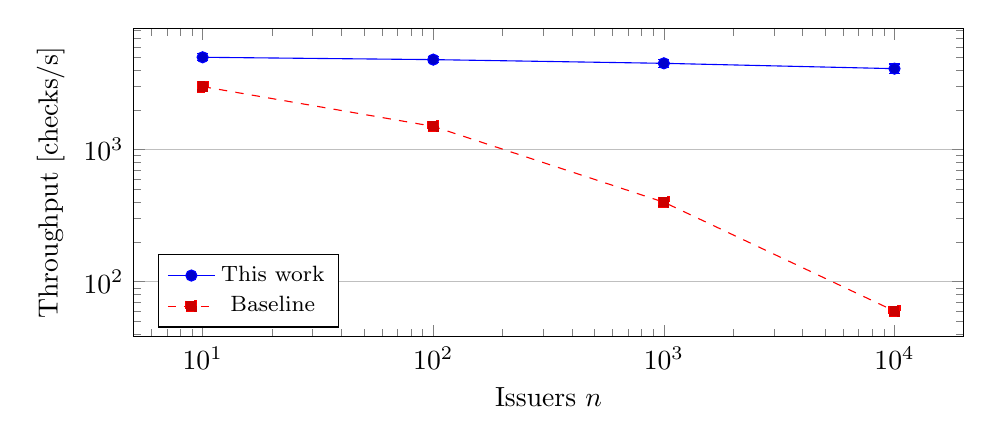
\begin{tikzpicture}
      \begin{axis}[width=\linewidth, height=55mm, xlabel={Issuers $n$}, xmode=log, ymode=log, ymajorgrids, legend style={font=\footnotesize}, ylabel={Throughput [checks/s]}, legend pos=south west]
        \addplot+[mark=*, error bars/.cd, y dir=both, y explicit]
          coordinates {(10,5000) +- (0,300) (100,4800) +- (0,250) (1000,4500) +- (0,300) (10000,4100) +- (0,350)};
        \addlegendentry{This work}
        \addplot+[mark=square*, dashed]
          coordinates {(10,3000) (100,1500) (1000,400) (10000,60)};
        \addlegendentry{Baseline}
      \end{axis}
    \end{tikzpicture}
    \caption{Throughput; higher is better.}\label{fig:guide:scalability-throughput}
  \end{subfigure}\hfill
  \begin{subfigure}[b]{0.48\linewidth}
    \centering
    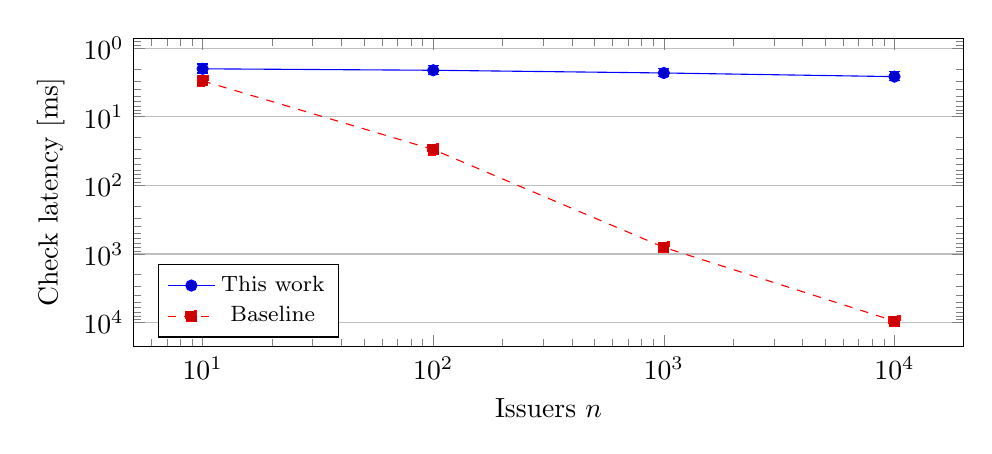
\begin{tikzpicture}
      \begin{axis}[width=\linewidth, height=55mm, xlabel={Issuers $n$}, xmode=log, ymode=log, ymajorgrids, legend style={font=\footnotesize}, ylabel={Check latency [ms]}, y dir=reverse, legend pos=south west]
        \addplot+[mark=*, error bars/.cd, y dir=both, y explicit]
          coordinates {(10,2) +- (0,0.3) (100,2.1) +- (0,0.3) (1000,2.3) +- (0,0.3) (10000,2.6) +- (0,0.4)};
        \addlegendentry{This work}
        \addplot+[mark=square*, dashed]
          coordinates {(10,3) (100,30) (1000,800) (10000,9500)};
        \addlegendentry{Baseline}
      \end{axis}
    \end{tikzpicture}
    \caption{Latency, axis reversed; lower is better, better is still up.}\label{fig:guide:scalability-time}
  \end{subfigure}
  \caption{Scalability as the number of issuers grows. Both panels put the better result on top. Mean of 10 runs with fresh issuer sets; error bars show one standard deviation.}
  \label{fig:guide:scalability}
\end{figure}

\begin{figure}[!ht]
  \centering
  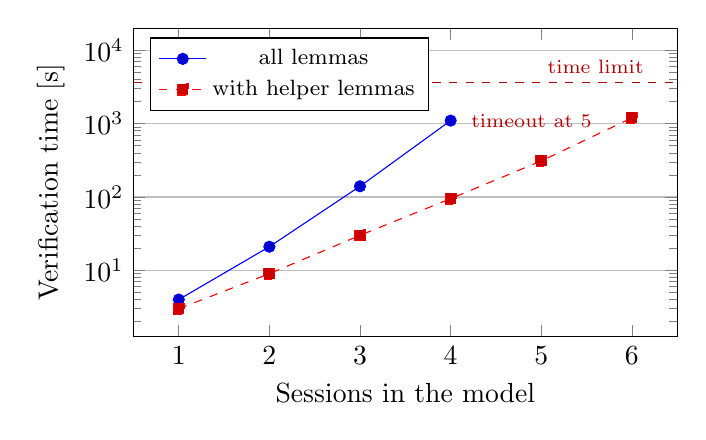
\begin{tikzpicture}
    \begin{axis}[width=0.7\linewidth, height=55mm, xlabel={Sessions in the model}, ylabel={Verification time [s]}, ymode=log, ymajorgrids, legend style={font=\footnotesize}, legend pos=north west, xmin=0.5, xmax=6.5, xtick={1,...,6}, ymax=20000]
      \draw[dashed, red!70!black] (axis cs:0.5,3600) -- (axis cs:6.5,3600) node[pos=0.85, above, font=\scriptsize] {time limit};
      \addplot+[mark=*] coordinates {(1,4) (2,21) (3,140) (4,1100)};
      \addlegendentry{all lemmas}
      \addplot+[mark=square*, dashed] coordinates {(1,3) (2,9) (3,30) (4,95) (5,310) (6,1200)};
      \addlegendentry{with helper lemmas}
      \node[font=\scriptsize, text=red!70!black, anchor=west] at (axis cs:4.12,1100) {timeout at 5};
    \end{axis}
  \end{tikzpicture}
  \caption{Track F sibling of \cref{fig:guide:scalability}: verification time of the registry model as it grows, with the time limit and the point where the prover stops. What grows is whatever your model is parametrised by: sessions, agents, the bound of a bounded check, or the number of lemmas.}
  \label{fig:guide:scalability-formal}
\end{figure}

\subsection[Robustness analysis (RQ3)]{Robustness analysis (RQ3)\skimmark}\label{app:chapters:robustness}
\guidebeat{how the system behaves when its assumptions are stressed: faults, attacks, load spikes, parameter changes}{the robustness table, with the setup of each perturbation}{the example under attack}{the threats to validity}
\textbf{Robustness is scored separately from scalability.} The review sheet gives 7--8 points on criterion E only if \enquote{a szerző skálázhatósági, robosztussági vizsgálatokat is elvégzett, mellyel igazolta, hogy rendszere ipari környezetben is megállja a helyét}: scalability \emph{and} robustness studies showing the system holds up in an industrial setting. Scalability alone does not earn it.
\textbf{Track S:} perturb the system on purpose and report what happens: \cref{tab:guide:robustness} lists the perturbations and their outcomes, \cref{fig:guide:robustness} shows how the system degrades and recovers during a fault, and how sensitive it is to its main parameter.
\textbf{Track F:} \cref{tab:guide:robustness-formal}: re-verify every property under a stronger adversary and with each assumption dropped, and report which still hold, which break, and the attack that breaks them.
\textbf{Track T:} \cref{tab:guide:robustness} with the tool's own perturbations: thresholds and parameters varied around their defaults, mutated or adversarial inputs (bugs injected on purpose: does the tool still find them), and benchmark instances from another source than the one it was developed on.

\begin{table}[!ht]
  \centering
  \caption{Robustness of the registry: each perturbation, what it tests, and how the registry behaved.}
  \label{tab:guide:robustness}
  {\small
  \begin{tabularx}{\linewidth}{>{\raggedright\arraybackslash}p{0.2\linewidth} >{\raggedright\arraybackslash}X >{\raggedright\arraybackslash}p{0.16\linewidth} >{\raggedright\arraybackslash}p{0.16\linewidth} >{\raggedright\arraybackslash}p{0.12\linewidth}}
    \toprule
    \textbf{Perturbation} & \textbf{What it tests} & \textbf{Expected} & \textbf{Observed} & \textbf{Recovery} \\
    \midrule
    Fault injection & One of four ledger nodes crashes during a burst of checks & checks go on, revocations wait & as expected, revocations 3.1\,s late & 12\,s \\
    Adversarial input & \Cref{thr:guide:holder} replays a week-old witness, 500 times & all rejected & all rejected & none needed \\
    Load spike & 10$\times$ the nominal check rate for 60\,s & latency within one round trip & p99 at 1.8$\times$ nominal & immediate \\
    Parameter sensitivity & The ledger timeout varied around its default & graceful & see \cref{fig:guide:robustness-sensitivity} & none needed \\
    \bottomrule
  \end{tabularx}
  }
\end{table}

\begin{table}[!ht]
  \centering
  \caption{Track F sibling of \cref{tab:guide:robustness}: each property re-verified under a stronger adversary and with each assumption dropped. \gapyes{} proved, \gapno{} attack found (the trace is in the appendix), \gappartial{} timed out.}
  \label{tab:guide:robustness-formal}
  {\small
  \begin{tabularx}{\linewidth}{l >{\raggedright\arraybackslash}X *{4}{>{\centering\arraybackslash}p{0.13\linewidth}}}
    \toprule
    & \textbf{Property} & \textbf{Base threat model} & \textbf{Registry key leaked} & \textbf{\ref{asm:guide:clock} dropped} & \textbf{Weaker signatures} \\
    \midrule
    \ref{g:guide:stale} & Bounded staleness (\cref{thm:guide:stale}) & \gapyes & \gapno & \gapno & \gappartial \\
    \ref{req:guide:private} & Holder privacy & \gapyes & \gapyes & \gapyes & \gapyes \\
    \bottomrule
  \end{tabularx}
  }
\end{table}

\begin{figure}[!ht]
  \centering
  \begin{subfigure}[b]{0.48\linewidth}
    \centering
    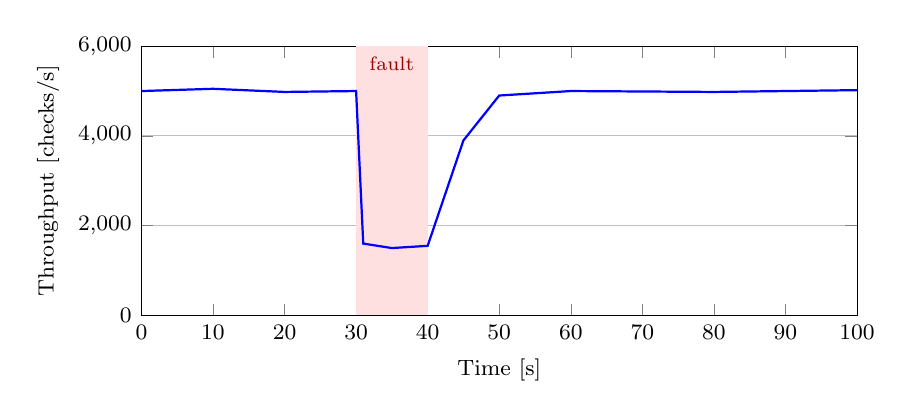
\begin{tikzpicture}
      \begin{axis}[width=0.88\linewidth, height=50mm, xlabel={Time [s]}, ylabel={Throughput [checks/s]}, ymin=0, ymax=6000, xmin=0, xmax=100, ymajorgrids, font=\footnotesize]
        \fill[red!12] (axis cs:30,0) rectangle (axis cs:40,6000);
        \node[font=\scriptsize, text=red!60!black] at (axis cs:35,5600) {fault};
        \addplot[mark=none, thick, blue] coordinates {(0,5000) (10,5050) (20,4980) (30,5000) (31,1600) (35,1500) (40,1550) (45,3900) (50,4900) (60,5000) (80,4980) (100,5020)};
      \end{axis}
    \end{tikzpicture}
    \caption{A ledger node fails between 30 and 40\,s: degradation and recovery.}\label{fig:guide:robustness-fault}
  \end{subfigure}\hfill
  \begin{subfigure}[b]{0.48\linewidth}
    \centering
    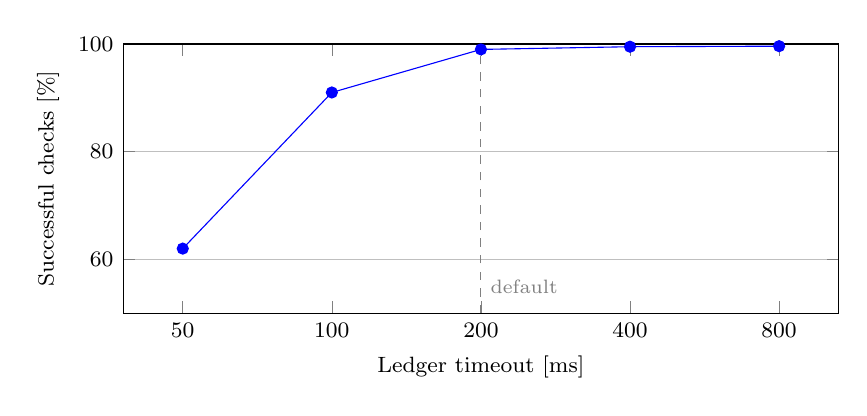
\begin{tikzpicture}
      \begin{axis}[width=0.88\linewidth, height=50mm, xlabel={Ledger timeout [ms]}, ylabel={Successful checks [\%]}, xmode=log, log basis x=2, xtick={50,100,200,400,800}, xticklabels={50,100,200,400,800}, ymin=50, ymax=100, ymajorgrids, font=\footnotesize]
        \draw[dashed, gray] (axis cs:200,50) -- (axis cs:200,100) node[pos=0.1, right, font=\scriptsize] {default};
        \addplot[mark=*, blue] coordinates {(50,62) (100,91) (200,99) (400,99.5) (800,99.6)};
      \end{axis}
    \end{tikzpicture}
    \caption{Sensitivity to the ledger timeout, around its default.}\label{fig:guide:robustness-sensitivity}
  \end{subfigure}
  \caption{Robustness: the registry during a node failure and under changes to its main parameter.}
  \label{fig:guide:robustness}
\end{figure}

\subsection{Threats to validity}\label{app:chapters:validity}
\guidebeat{what could make the results wrong or not generalise, and what was done about each}{the mitigations}{whether the example is representative of real use}{related work}
For the registry: the issuer sets are synthetic, and every measurement ran on one machine. Say for each threat what was done about it, and what was not.

%----------------------------------------------------------------------------
\section{Related work and gap analysis}\label{app:chapters:related}
%----------------------------------------------------------------------------
\textbf{Criteria B/2 (0--4) and D/1 (0--5).} This chapter comes after the evaluation, as in research papers: the reader now knows what you built and measured, so each comparison can point to a concrete result instead of a promise.
\textbf{Novelty:} place the related work on a positioning figure, compare the closest approaches against the requirements in a gap matrix, and end with the gap only your work fills.
\textbf{Relevance:} include current industrial solutions and recent research, so the gap is visibly open today.

\textbf{In the sheet's words.} The top of B/2: \enquote{3--4: újszerű ipari megoldások és kutatási eredmények (a dolgozat -- az újszerű ipari megoldásokon túl -- bemutatja a dolgozat témakörében releváns kutatási eredményeket a szakterületen)}; the step below, \enquote{2: újszerű ipari megoldások vagy közismert kutatási eredmények}, is where a chapter without recent research lands. D/1 falls to \enquote{1--2: ismert (a kutatási terület szakirodalomban számos megoldás ismert a tárgyalt problémára, és ezek „másolás jellegű” alkalmazására került sor a dolgozatban)} or \enquote{3--4: inkrementális (értékes inkrementális kontribúció, létező megoldások apró továbbfejlesztése)} when the gap matrix shows a close neighbour; argue the difference here.

\subsection{Comparison criteria}\label{app:chapters:comparison-criteria}
The comparison uses the requirements of the introduction, here \cref{req:guide:timely,req:guide:offline,req:guide:private}. Add criteria only if a reader would ask about them, such as maturity or license.

\subsection[Existing approaches]{Existing approaches\skimmark}\label{app:chapters:existing-approaches}
\guidebeat{how each family of approaches works and where it falls short}{citations, the positioning figure and the gap matrix}{what each approach does with the example}{the gap}
Group the related work into families and discuss each family against the requirements. \Cref{fig:guide:positioning} places every approach on the two properties that separate them most, so the gap shows as the one empty cell; \cref{tab:guide:related} then compares the closest approaches requirement by requirement in a gap matrix: a reader should see the gap from the matrix alone, as the one column where every row is met.

The positioning figure: the related work as dots on two axes of three levels each, this work as the star in the cell no existing approach reaches, and an arrow from the closest approach that says what this work adds. Choose the two properties that separate the approaches most: two requirements, or two that each sum up several. Name the levels in words, never low, medium and high.
\begin{runningexample}[elsewhere]
With Approach C, the closest one, the employer checks offline against a list fetched in the morning, so a diploma revoked at noon passes every check until the next fetch: it fails \cref{req:guide:timely}.
\end{runningexample}

\begin{figure}[!ht]
  \centering
  \begin{tikzpicture}[
      work/.style={circle, fill=gray!60!black, draw=white, line width=0.5pt, inner sep=0pt, minimum size=2.3mm},
      wlbl/.style={anchor=west, font=\footnotesize, inner sep=1pt, fill=white},
      wnote/.style={anchor=north west, font=\scriptsize\itshape, text=gray!70!black, inner sep=1pt, fill=white},
      tick/.style={font=\footnotesize\bfseries, align=center},
      sub/.style={font=\scriptsize\itshape, text=gray!80!black, align=center}]
    \def\cA{1.8}\def\cB{6.0}\def\cC{10.2} % columns: the levels of the second property
    \def\rA{0.9}\def\rB{2.6}\def\rC{4.7}  % rows: the levels of the first property
    \def\xmax{14.6}\def\ymax{5.8}
    \fill[blue!8, rounded corners=4pt] ({(\cB+\cC)/2},3.95) rectangle (\xmax,\ymax-0.15); % the gap
    \foreach \y in {\rA,\rB,\rC} \draw[gray!30, dashed] (0,\y) -- (\xmax,\y);
    \foreach \x in {\cA,\cB,\cC} \draw[gray!30] (\x,0) -- (\x,\ymax-0.15);
    \draw[line width=0.9pt, -{Stealth[length=2.6mm]}] (0,0) -- (\xmax+0.3,0);
    \draw[line width=0.9pt, -{Stealth[length=2.6mm]}] (0,0) -- (0,\ymax+0.2);
    \node[anchor=south west, inner sep=0pt, font=\footnotesize] at (0.15,\ymax+0.05)
      {\textbf{How soon a revocation is seen} $\uparrow$\enspace\textit{how far an approach meets \cref{req:guide:timely}}};
    \node[anchor=north east, align=right, font=\footnotesize] at (\xmax+0.3,-0.85)
      {\textbf{What a check needs} $\rightarrow$\\\textit{\scriptsize how far it meets \cref{req:guide:offline}}};
    \foreach \y/\name/\what in {\rC/within $\delta$/bounded by the clocks, \rB/minutes/a cache's lifetime, \rA/days/the next list} {%
      \draw (-0.08,\y) -- (0.08,\y);
      \node[tick, anchor=south east] at (-0.15,\y+0.02) {\name};
      \node[sub, anchor=north east] at (-0.15,\y+0.02) {\what};
    }
    \foreach \x/\name/\what in {\cA/the issuer/asked at every check, \cB/a fresh list/fetched before the check, \cC/nothing/the credential alone} {%
      \draw (\x,-0.08) -- (\x,0.08);
      \node[tick, anchor=north] at (\x,-0.15) {\name};
      \node[sub, anchor=north] at (\x,-0.5) {\what};
    }
    \node[work] (a) at (\cA,\rC) {};
    \node[wlbl] at (a.east) {Approach A};
    \node[wnote] at (\cA+0.05,\rC-0.2) {online status checks};
    \node[work] (d) at (\cB,\rB) {};
    \node[wlbl] at (d.east) {Approach D};
    \node[work] (b) at (\cC,\rA) {};
    \node[wlbl] at (b.east) {Approach B};
    \node[work] (c) at (\cC,\rB) {};
    \node[wlbl] at (c.east) {Approach C};
    \node[wnote] at (\cC+0.05,\rB-0.2) {the closest approach};
    % this work, reached from the closest approach
    \draw[blue!60!black, line width=1.2pt, dashed, -{Stealth[length=2.6mm]}] (c.north) -- (\cC,\rC-0.32);
    \node[star, star points=5, star point ratio=2.3, minimum size=6.5mm, inner sep=0pt,
          fill=blue!60!black, draw=white, line width=0.6pt] (tw) at (\cC,\rC) {};
    \node[anchor=west, font=\normalsize\bfseries, text=blue!60!black, inner sep=1pt] at ([xshift=2pt]tw.east) {This work};
    \node[anchor=north west, font=\scriptsize\itshape, text=blue!60!black, inner sep=1pt] at (\cC+0.38,\rC-0.22) {a registry with bounded staleness};
    \node[anchor=west, font=\footnotesize, text=blue!60!black, align=left, inner sep=1pt] at (\cC+0.2,3.35)
      {+ values fresh within $\delta$\\+ checked without the issuer};
  \end{tikzpicture}
  \caption{Positioning figure: the related work on the two properties that separate it most. Grey dots are existing approaches; the blue star is this work, in the cell no existing approach reaches, and the dashed arrow starts at the closest approach and says what this work adds.}
  \label{fig:guide:positioning}
\end{figure}

\begin{table}[!ht]
  \centering
  \caption{Gap matrix: each requirement against the closest approaches. \gaplegend. Cells for this work point to the evaluation result that backs them.}
  \label{tab:guide:related}
  \renewcommand{\arraystretch}{1.3}
  \begin{tabularx}{\linewidth}{l X c c c c}
    \toprule
    & \textbf{Requirement} & \textbf{Approach A} & \textbf{Approach B} & \textbf{Approach C} & \textbf{This work} \\
    \midrule
    \ref{req:guide:timely}  & Timely revocation & \gapyes & \gapno  & \gappartial & \gapyes\,(\cref{thm:guide:stale}) \\
    \ref{req:guide:offline} & Offline checks    & \gapno  & \gapyes & \gapyes     & \gapyes\,(\cref{rq:guide:correct}) \\
    \ref{req:guide:private} & Holder privacy    & \gapno  & \gapyes & \gappartial & \gapyes\,(\cref{rq:guide:correct}) \\
    \bottomrule
  \end{tabularx}
\end{table}

\subsection{Gap}\label{app:chapters:gap}
\guidebeat{the gap in one sentence, closed by this work}{the gap matrix and the results of the evaluation}{the scenario as the case only this work handles}{the conclusion}
One paragraph that states the gap in one sentence, based on the positioning figure and the gap matrix, and shows with the results of the evaluation that this work closes it. This paragraph is the novelty argument. Here: no existing approach makes a revocation visible within $\delta$ to a verifier that asks nobody, and the registry does, by \cref{thm:guide:stale} and the measurements of \cref{rq:guide:correct}.

%----------------------------------------------------------------------------
\section{Conclusion and future work}\label{app:chapters:conclusion}
%----------------------------------------------------------------------------
\textbf{Criterion E.} This chapter is where the reviewer checks that the contributions promised in the introduction were delivered and evaluated. Many readers open it right after the abstract, before the rest, so it leads with what was achieved. Close with limitations and concrete future work.
\textbf{Novelty:} restate each contribution from the introduction with the gap it closes.
\textbf{Correctness:} restate each with the proof or measurement behind it.

\textbf{In the sheet's words.} The top of E: \enquote{7--8: teljeskörű -- A bevezetés megfelelő és az elért eredmények pontosak és teljesek, az értékelés megalapozott}.

\subsection[Summary]{Summary\skimmark}\label{app:chapters:summary}
\guidebeat{each contribution and its evidence}{the chapters behind C1--C3}{the example, now solved}{the limitations}
One paragraph per contribution, each with its evidence: here \cref{c:guide:model} with \cref{thm:guide:stale}, \cref{c:guide:registry} with the archived artifact, and \cref{c:guide:eval} with the answers to \cref{rq:guide:correct,rq:guide:scale,rq:guide:robust}. The box closes the scenario opened in the introduction, in one or two sentences.
\begin{runningexample}[in retrospect]
The withdrawn diploma no longer gets anyone hired: the employer's offline check rejects it within $\delta$ of its revocation, and the university never learns that the employer asked.
\end{runningexample}

\subsection[Limitations and future work]{Limitations and future work\skimmark}\label{app:chapters:future}
\guidebeat{what is still open, and the next step that would lift each limitation}{the threats to validity}{what the example does not cover}{the venue to target next}
Each limitation is a tagged item, so the future work can name the one it lifts.
\begin{limitations}
  \item\label{lim:guide:synthetic} \textbf{Synthetic workloads.} The evaluation uses synthetic issuer sets only.
  \item\label{lim:guide:force} \textbf{No forced revocation.} The registry cannot make an issuer revoke a credential it should.
\end{limitations}
